\documentclass[12pt,UTF8]{ctexbook}
\usepackage{ctex}
\usepackage{array}
\usepackage{graphicx}
\usepackage{wrapfig}
\usepackage[table,dvipsnames]{xcolor}
\usepackage{tabularx}
\usepackage{amsmath}
\usepackage{amssymb}
\usepackage{xfrac}
\usepackage{eucal}
\usepackage{titlesec}
\usepackage{amsthm}
\usepackage{tikz-cd}
\usepackage{enumitem}
\usepackage{verbatim}
\usepackage{fontspec,xunicode,xltxtra}
\usepackage{xeCJK} 

\definecolor{gl}{RGB}{246, 252, 240}
\definecolor{gd}{RGB}{236, 244, 230}
\definecolor{bg}{RGB}{242, 244, 228}


\setCJKmainfont[BoldFont=STZhongsong]{STSong}
\setCJKmonofont{simkai.ttf} % for \texttt
\setCJKsansfont{simfang.ttf} % for \textsf
\setlength\parskip{8pt}
\setlength{\fboxsep}{12pt}
\renewcommand\thesection{\arabic{chapter}.\arabic{section}}
\newtheorem{df}{定义}[section] 
\newtheorem{pp}{命题}[section]
\newtheorem{tm}{定理}[section]
\newtheorem{ex}{例子}[section]
\newtheorem{et}{例题}[section]
\newtheorem{sk}{思考}[section]
\newtheorem*{so}{解答}
\newenvironment{proof2}{\paragraph{\textbf{证明:}}}{\hfill$\square$}
\newtheorem{xt}{习题}[section]
\newtheorem{cor}{推论}[pp]
% 列举环境的行间距
\setenumerate[1]{itemsep=0pt,partopsep=0pt,parsep=0pt,topsep=0pt}
\setitemize[1]{itemsep=0pt,partopsep=0pt,parsep=0pt,topsep=0pt}
\setdescription{itemsep=0pt,partopsep=0pt,parsep=0pt,topsep=0pt}
% 章节字体大小
\titleformat{\section}{\zihao{-2}\bfseries}{ \thesection }{16pt}{}
% 封面
\title{\zihao{0} \bfseries 第三册}
\author{\zihao{2} \texttt{大青花鱼}}
% \date{\bfseries\today}
\date{}
% 正文
\begin{document}
\maketitle
\tableofcontents
\newpage


\chapter{数列的极限}

\section{极限的基本性质}
我们来考察以下数列:
$$ 0,\,\, \frac{1}{2}, \,\,\frac{2}{3},\,\, \frac{3}{4}, \,\,\frac{4}{5}, \,\,\frac{5}{6}, \cdots $$
它的通项公式是$a_n = \frac{n-1}{n}$。
把数列的前几项在数轴上标出来,我们发现:
随着$n$不断增大,$a_n$不断变大,不断向着$1$靠拢。

数列$\{a_n\}$各项随着$n$增大,不断接近$1$。
虽然数列任一项都不等于$1$,但我们不难产生这样的想法:随着$n$增大,$a_n$的值任意接近于$1$。

怎样严谨地表达这个想法呢?我们使用“有求必应”和“一路全真”的结构,把上面的想法用更具体的方式来描述。
直观来看,我们考察以$1$为中心的区间$[1-r,1+r]$,
无论这个区间多么小,到了一定的$n$以后,所有的$a_n$都会落在这个区间里。

用二元命题$Q(r, n)$表示“$a_n$落在区间$[1-r,1+r]$里”。
用类似“有求必应”的结构,以上的想法可以写成:
$$\forall r > 0, \,\,\, \exists n,  \,\,\, \mbox{使得} \forall \,\, m \geqslant n, \,\,\, Q(r, n)\mbox{成立。}$$
这个结构比“有求必允”结构要求更高。它不仅要求“必允”,而且一旦“允”了,就要求之后“一路全真”。
用表格来表示这个结论:

\begin{figure}[h] %this figure will be at the right
    % \vspace{4pt}
    \centering
    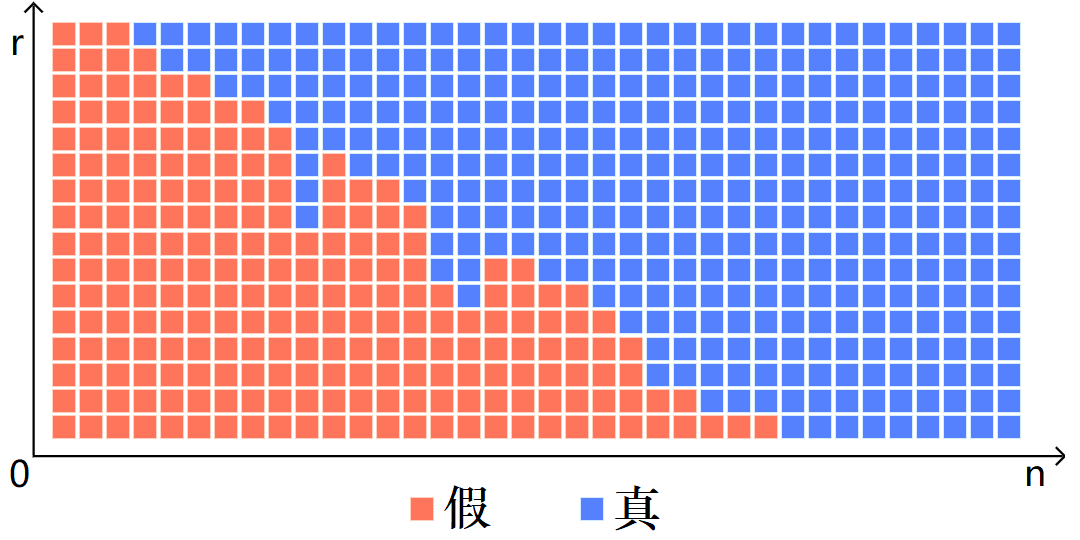
\includegraphics[width=0.64\textwidth]{数列极限2.png}
\end{figure}

每格颜色对应$Q(r, n)$的真假。每一行对应一个正数$r$,每一列对应数列的一个下标$n$。我们的想法是:
不论$r>0$是多少,它对应的行中,$Q(r, n)$必然从某一列起全为真。

我们把$1$称为数列$\{a_n\}$的\textbf{极限}。对一般数列来说,我们定义:
\begin{df}\textbf{数列的极限} \\
设有无穷数列$\{a_n\}$。如果有某个数$x$,使得
$$ \forall r > 0, \,\,\, \exists n,  \,\,\, \mbox{使得} \,\,\, \forall \,\, m \geqslant n, \,\,\, - r \leqslant a_m - x \leqslant r. $$
就说$\{a_n\}$有极限$x$,或$x$是$\{a_n\}$的极限,或$\{a_n\}$趋于$x$,记作
$$\lim_{n\to\infty} a_n = x.$$
\end{df}

\begin{figure}[h] %this figure will be at the right
    \vspace{-14pt}
    \centering
    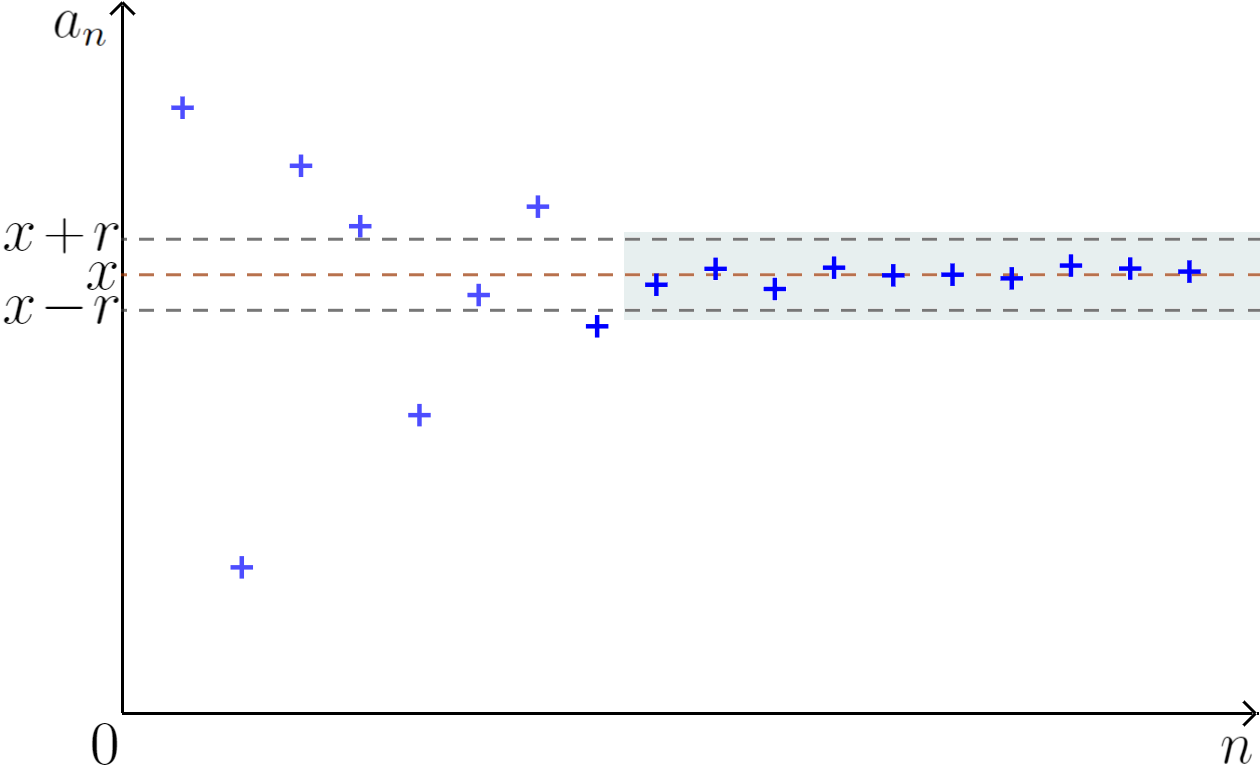
\includegraphics[width=0.54\textwidth]{数列极限1.png}
    \caption*{\texttt{从某一项开始,数列的值总落在区间}$[x-r,x+r]$\texttt{中}}
\end{figure}

\begin{et}
数列$\{a_n\}$的通项是$a_n = \frac{1}{n^2}$,它是否有极限?如果有极限,极限是多少?    
\end{et}
\begin{so}
    $\{a_n\}$每项都是正数。
    $$a_{n} \div a_{n+1} = \frac{1}{n^2} \div \frac{1}{(n+1)^2} = \frac{(n+1)^2}{n^2} = 1 + \frac{2n+1}{n^2} > 1,$$
    所以$\{a_n\}$是单调递减数列。从数轴上看,$\{a_n\}$不断趋近于$0$。猜测它有极限$0$。\\
    设$r>0$,考察区间$[-r,r]$。设$n_r$是大于等于$\frac{1}{\sqrt{r}}$的最小正整数,
    那么,只要$n \geqslant n_r$,就有$n^2 \geqslant n_r^2 \geqslant \frac{1}{r}$,
    于是$0 \leqslant \frac{1}{n^2} \leqslant r$。因此,$\forall r > 0$,$\exists n_r$,
    使得$\forall m \geqslant n_r$,$ -r  \leqslant a_m - 0 \leqslant r$。这说明$\{a_n\}$有极限$0$。    
\end{so}

不难看出,极限是构造出来的。因此,从定义出发,我们可以说某个数是某数列的极限。
反过来,一个数列有极限,它的极限是否只能有一个呢?答案是肯定的。我们可以用反证法来证明。

反设某数列$\{a_n\}$有两个极限$x_1, x_2$。不妨设$x_1 < x_2$。直觉上,$n$足够大的时候,$a_n$在数轴上离$x_1, x_2$都很近,
到两点的距离比$x_2 - x_1$的一半都小,加起来就小于$x_2 - x_1$,于是就产生矛盾了。

具体来说,记$\delta = \frac{x_2 - x_1}{2}$为两点距离的一半。选一个小于$\delta$的正数$r$。
按照极限的定义,有正整数$n_1, n_2$使得:
\begin{align}
    \forall m \geqslant n_1 , \,\,\,& -r \leqslant a_m - x_1 \leqslant r , \notag \\
    \forall m \geqslant n_2 , \,\,\,& -r \leqslant a_m - x_2 \leqslant r . \notag 
\end{align}
于是,选一个比$n_1,n_2$都大的$m$,比如$m=n_1+n_2$,这时$a_m - x_1 \leqslant r$,$x_2 - a_m \leqslant r$。
加起来就得到:
$$x_2 - x_1 \leqslant 2r < 2\delta = x_2 - x_1.$$
矛盾!因此,\textbf{数列如果有极限,只能有一个。}

设数列$\{a_n\}$有极限$x$。我们把它每一项减去$x$(或者说让数列减去常数列$\{x\}$),
得到的数列$\{a_n - x\}$趋于$0$。所以,任何有极限的数列,都可以看做一个趋于$0$的数列加上它的极限。
我们把趋于$0$的数列称为\textbf{无穷小}。任何有极限的数列,都是它的极限加上无穷小。

极限描述了数列的项在“远处”的特征。我们把数列下标超过一定限度后的特征称为数列的\textbf{大体行为}。
有极限的数列,我们可以用极限来刻画数列的大体行为(落在极限“附近”)。
没有极限的数列,大体行为有什么特征呢?

我们来看另一个数列:
$$ 1,\,\,2,\,\,3,\,\,4,\,\,5,\cdots $$
它是正整数数列,通项为$a_n = n$。不难看出,它没有极限。因为对任何实数$x$来说,
令$n_x$为大于$x$的最小正整数,那么从$n_x+1$开始的项都比$x$大至少$1$,
无法落到$x$附近的小区间里面。可以说,随着$n$增大,$a_n$会比任何数都大。

如何严谨描述这个想法呢?我们仍然可以用“有求必应”的结构,把以上想法写成:
$$ \forall x, \,\,\, \exists n, \,\,\,\mbox{使得} \,\,\,\forall \,\, m \geqslant n,,\,\,\, a_m \geqslant x.$$
直观来看,随着$n$增大,从某一项开始,$a_n$会落到数轴任何给定点$x$的右边。
我们把这个性质称为数列\textbf{趋于正无穷大}。同理,可以定义数列\textbf{趋于负无穷大}:
$$\forall x, \,\,\, \exists n, \,\,\,\mbox{使得}\,\,\,\forall \,\, m \geqslant n,,\,\,\, a_m \leqslant x.$$
直观来看,随着$n$增大,从某一项开始,$a_n$会落到数轴任何给定点$x$的左边。

\begin{wrapfigure}[9]{r}{0.33\textwidth} %this figure will be at the right
    \vspace{-48pt}
    \flushright
    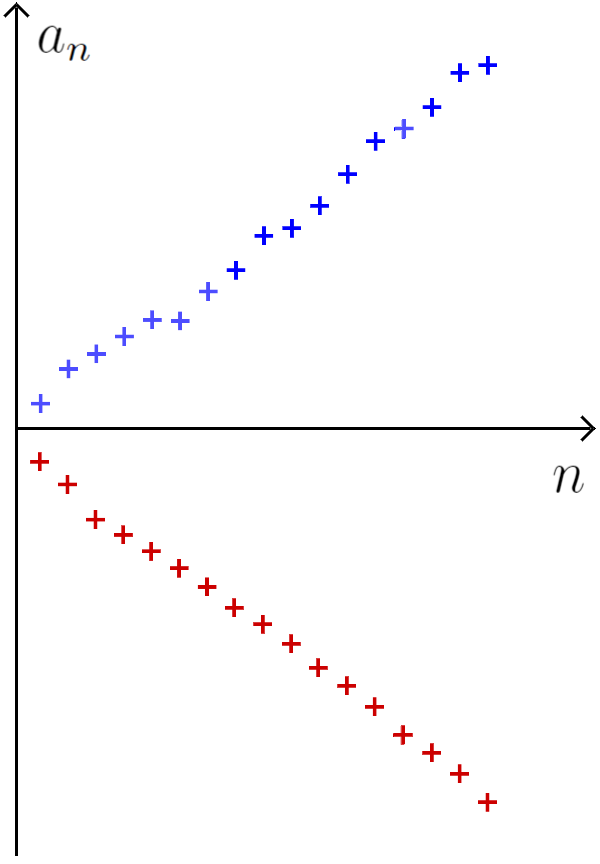
\includegraphics[width=0.32\textwidth]{数列无穷大1.png}
    \caption*{\texttt{趋于无穷大的数列}}
\end{wrapfigure}

我们也把有这两个性质的数列简称为\textbf{正无穷大}和\textbf{负无穷大}。

\begin{et}
    设数列$\{\frac{1}{n}\}$的部分和数列为$\{a_n\}$,证明:$\{a_n\}$趋于正无穷大。
\end{et}
\begin{proof2}
    按照定义,$ a_n = 1 + \frac{1}{2} + \cdots + \frac{1}{n}$。\\
    $a_{n+1} - a_n = \frac{1}{n+1} > 0$,所以$\{a_n\}$单调递增。\\
    对任意实数$x$,我们需要找到相应的$n$,使得$\forall m \geqslant n$,$a_m \geqslant x$。
    由于$\{a_n\}$单调递增,只要某一项$a_n \geqslant x$,它之后的项都大于等于$x$。
    因此,只需要找到$n$使得$a_n \geqslant x$即可。\\
    如果$x \leqslant 1$,那么$n=1$即满足要求。\\
    如果$x > 1$,设$M$是大于$x$的最小整数,考虑$n = 2^{2M}$。下面证明$a_{2^{2M}}>x$。\\
    $$ a_{2^{2M}} = a_{2^0} + \sum_{i=1}^{2M}a_{2^i} - a_{2^{i-1}}.$$
    \begin{align}
        \forall \,\, i\in[1\ldots 2M],\,\,\, a_{2^i} - a_{2^{i-1}} &= \frac{1}{2^{i-1}+1} + \frac{1}{2^{i-1}+2} + \cdots + \frac{1}{2^{i}} \notag \\
        &\geqslant \frac{1}{2^{i}} + \frac{1}{2^{i}} + \cdots + \frac{1}{2^{i}} \notag \\
        &= \frac{2^{i-1}}{2^{i}} = \frac{1}{2}. \notag
    \end{align}
    $$ \mbox{所以}\quad  a_{2^{2M}} \geqslant a_1 + \frac{1}{2} \cdot (2M - 1) = M + \frac{1}{2} > x. $$
    这就证明$\{a_n\}$趋于正无穷大。
\end{proof2}

\begin{sk}
    \mbox{} \\
    \indent 1. 张三在判定数列$\{a_n\}$的极限时写到:数$x$满足:
    $$ \forall r > 0, \,\,\, \exists n,  \,\,\, \mbox{使得} \forall \,\, m > n \,\,\, \mbox{都有} x - r < a_m < x + r. $$
    \indent 因此$\{a_n\}$有极限$x$。他的说法对吗?\\
    \indent 2. 李四在判定数列$\{a_n\}$的极限时写到:数$x$满足:
    $$ \forall r > 0, \,\,\, \exists n,  \,\,\, \mbox{使得} \forall \,\, m > n \,\,\, \mbox{都有} x - 2r \leqslant a_m \leqslant x + 2r. $$
    \indent 因此$\{a_n\}$有极限$x$。他的说法对吗?\\
    \indent 3. 一般数列除了有极限和趋于正负无穷大,还可能有什么大体行为?\\
    \indent 4. 单调数列除了有极限和趋于正负无穷大,还可能有什么大体行为?
\end{sk}

\begin{xt}
    \mbox{} \\
    \indent 1. 以下数列是否有极限?如果有极限,是多少?\\
    \indent\indent 1.1. $\{2^{1-n}\}$ \\
    \indent\indent 1.2. $\{(-1)^{n-1}\frac{n+1}{3n+1}\}$ \\
    \indent\indent 1.3. $\{1 - \frac{1}{n^3+1}\}$ \\
    \indent 2. 以下数列是否趋于无穷大?\\
    \indent\indent 2.1. $\{2^{n}\}$ \\
    \indent\indent 2.2. $\{n^2\}$ \\
    \indent\indent 2.3. $\{\frac{2^n}{n^2}\}$\\
    \indent 3. 如果数列$\{a_n\}$趋于$x$,证明:$\{a_n\}$的任何子列趋于$x$。
\end{xt}

\section{极限的运算}
我们已经学习了数列的运算。数列之间可以做加法、减法、乘法。
如果数列$\{a_n\}$、$\{b_n\}$有极限,它们的和、差、乘积是否有极限?
答案是肯定的,并且符合我们的直觉:
\begin{tm}
    若数列$\{a_n\}$趋于$a$,$\{b_n\}$趋于$b$,则
    \begin{align}
        \lim_{n\to\infty} a_n \pm b_n &= a \pm b, \notag \\
        \lim_{n\to\infty} a_n \cdot b_n &= a \cdot b. \notag 
    \end{align}
\end{tm}
特别地,令$\{b_n\}$是常数列,就得到数乘对极限的影响:若数列$\{a_n\}$趋于$a$,则
$$ \forall \,\, t \in \mathbb{R}, \,\,\,  \lim_{n\to\infty} t \cdot a_n = ta. $$
\begin{proof2}
    \mbox{} \\
    首先证明极限的加法:设数列$\{a_n\}$趋于$a$,$\{b_n\}$趋于$b$。按照定义,$\forall r > 0$,
    由于$\frac{r}{2}>0$,总有正整数$n_a, n_b$,使得
    \begin{align}
        \forall \,\, m \geqslant n_a, \,\,\, & - \frac{r}{2} \leqslant a_m - a \leqslant \frac{r}{2}, \notag \\
        \forall \,\, m \geqslant n_b, \,\,\, & - \frac{r}{2} \leqslant b_m - b \leqslant \frac{r}{2}, \notag 
    \end{align}
    因此,
    \begin{align}
        \forall \,\, m \geqslant n_a + n_b, \,\,\, & -r = - \frac{r}{2} - \frac{r}{2} \leqslant a_m + b_m - a - b \leqslant \frac{r}{2} + \frac{r}{2} = r \notag 
    \end{align}
    于是数列$\{a_n\} + \{b_n\}$趋于$a + b$。\\
    接下来证明极限的数乘:设$t$为实数,数列$\{a_n\}$趋于$a$,则数列$\{t\cdot a_n\}$趋于$ta$。
    这样,数列$\{a_n\} - \{b_n\}$可以看作$\{a_n\} + \{-b_n\}$,因而趋于$a - b$。\\
    分两种情况讨论。如果$t=0$,那么$\{t\cdot a_n\} = \{0\}$,显然趋于$0$,也就是$ta$。
    如果$t \neq 0$,按照定义,对$\forall r > 0$,由于$\frac{r}{t} > 0$,总有正整数$n$使得
    $$ \forall \,\, m \geqslant n, \,\,\, a - \frac{r}{t} \leqslant a_m \leqslant a + \frac{r}{t}. $$
    因此
    $$ \forall \,\, m \geqslant n, \,\,\, ta - r \leqslant t\cdot a_m \leqslant ta + r. $$
    这就说明数列$\{t\cdot a_n\}$趋于$ta$。\\
    最后证明极限的乘法:设数列$\{a_n\}$趋于$a$,$\{b_n\}$趋于$b$。按照定义,$\forall r > 0$,
    由于$\sqrt{r}>0$,总有正整数$n_a, n_b$,使得
    \begin{align}
        \forall \,\, m \geqslant n_a, \,\,\, & - \sqrt{r} \leqslant a_m - a \leqslant \sqrt{r}, \notag \\
        \forall \,\, m \geqslant n_b, \,\,\, & - \sqrt{r} \leqslant b_m - b \leqslant \sqrt{r}, \notag 
    \end{align}
    因此
    \begin{align}
        \forall \,\, m \geqslant n_a + n_b, \,\,\, & (a_m - a)(b_m - b) \leqslant \left(\sqrt{r}\right)^2 = r  \notag \\
        & -(a_m - a)(b_m - b) \leqslant \left(\sqrt{r}\right)^2 = r,  \notag \\
        \mbox{即 }\quad & - r \leqslant (a_m - a)(b_m - b) \leqslant r. \notag 
    \end{align}
    这说明数列$\{(a_n - a)(b_n - b)\}$趋于$0$。而$\{b\cdot a_n\}$和$\{a \cdot b_n\}$都趋于$ab$,
    常数列$\{ab\}$也趋于$ab$,所以根据前面证明的极限加减法,数列
    $$\{a_nb_n\} = \{(a_n - a)(b_n - b)\} + \{b\cdot a_n\} + \{a \cdot b_n\} - \{ab\}$$
    趋于$0 + ab + ab - ab = ab$。
\end{proof2}

四则运算中,加法、减法、乘法都可以对数列的极限做运算。那么除法是否可以呢?
具体来说,若数列$\{a_n\}$趋于$a$,$\{b_n\}$趋于$b$,是否有$\{\frac{a_n}{b_n}\}$趋于$\frac{a}{b}$?

显然,$b=0$的时候,$\frac{a}{b}$无定义,所以排除$\{b_n\}$趋于$0$的情况。如果$b$不等于$0$,
答案大致是肯定的。$\{\frac{a_n}{b_n}\}$趋于$\frac{a}{b}$。
当然,我们要先“剪掉”$\{b_n\}$最开始一些离$b$比较远的项,确保剩下的项都不等于$0$,这样才好定义$\frac{a_n}{b_n}$。
然后可以用类似证明极限乘法的方法,证明$\{\frac{1}{b_n}\}$趋于$\frac{1}{b}$,
这样,$\{\frac{a_n}{b_n}\}$可以看作$\{a_n \cdot \frac{1}{b_n}\}$,因而趋于$\frac{a}{b}$。

\begin{sk}
    \mbox{} \\
    \indent 1. 如果数列$\{a_n\}$有极限$a$,$\{b_n\}$趋于无穷大,它们的和、差、乘积、商数列是否有极限?是否趋于无穷大?\\
    \indent 2. 如果数列$\{a_n\}$、$\{b_n\}$都趋于无穷大,它们的和、差、乘积、商数列有什么特性?
\end{sk}

\begin{xt}
    \mbox{} \\
    \indent 1. 如果数列$\{a_n\}$有极限$a$,$\{b_n\}$趋于无穷大,它们的和、差、乘积、商数列是否有极限?是否趋于无穷大?\\
    \indent 2. 如果数列$\{a_n\}$、$\{b_n\}$都趋于无穷大,它们的和、差、乘积、商数列有什么特性?
\end{xt}

\section{关于数列极限的一些定理}

\end{document}